% Template for Cogsci submission with R Markdown

% Stuff changed from original Markdown PLOS Template
\documentclass[10pt, letterpaper]{article}

\usepackage{cogsci}
\usepackage{pslatex}
\usepackage{float}
\usepackage{caption}

% amsmath package, useful for mathematical formulas
\usepackage{amsmath}

% amssymb package, useful for mathematical symbols
\usepackage{amssymb}

% hyperref package, useful for hyperlinks
\usepackage{hyperref}

% graphicx package, useful for including eps and pdf graphics
% include graphics with the command \includegraphics
\usepackage{graphicx}

% Sweave(-like)
\usepackage{fancyvrb}
\DefineVerbatimEnvironment{Sinput}{Verbatim}{fontshape=sl}
\DefineVerbatimEnvironment{Soutput}{Verbatim}{}
\DefineVerbatimEnvironment{Scode}{Verbatim}{fontshape=sl}
\newenvironment{Schunk}{}{}
\DefineVerbatimEnvironment{Code}{Verbatim}{}
\DefineVerbatimEnvironment{CodeInput}{Verbatim}{fontshape=sl}
\DefineVerbatimEnvironment{CodeOutput}{Verbatim}{}
\newenvironment{CodeChunk}{}{}

% cite package, to clean up citations in the main text. Do not remove.
\usepackage{cite}

\usepackage{color}

% Use doublespacing - comment out for single spacing
%\usepackage{setspace}
%\doublespacing


% % Text layout
% \topmargin 0.0cm
% \oddsidemargin 0.5cm
% \evensidemargin 0.5cm
% \textwidth 16cm
% \textheight 21cm

\title{Postural changes mediate children's visual access to social information}


\author{{\large \bf Alessandro Sanchez} \\ \texttt{author1@university.edu} \\ Department of Psychology \\ Stanford University \And {\large \bf Bria Long} \\ \texttt{bria@stanford.edu} \\ Department of Psychology \\ Stanford University
    \And {\large \bf Ally Kraus} \\ \texttt{bria@stanford.edu} \\ Department of Psychology \\ Stanford University
    \And {\large \bf Michael C. Frank} \\ \texttt{mcfrank@stanford.edu} \\ Department of Psychology \\ Stanford University}

\begin{document}

\maketitle

\begin{abstract}


\textbf{Keywords:}
social cognition; face-perception; infancy; locomotion; head-cameras
\end{abstract}

\section{Introduction}\label{introduction}

Children are remarkably skilled language learners, connecting arbitrary
labels (``cup'') with specific visual concepts at a rapid pace through
the first two years of life. However, children do not learn words in a
vacuum but rather in a rich social environment, where social cues
provided by speakers (e.g., eye-gaze) provide strong scaffolding for
this learning process. Further, children's ability to effectively
process these social cues may be a key factor in their early language
development. In a longitudinal study, children's level of joint
engagement with their mother was found to predict both their receptive
and productive vocabularies (Carpenter, Nagell, \& Tomasello (1998)).
More recently, 10 month-olds who follow an adult's gaze in an
experimental context have larger vocabularies at 18 months (Brooks \&
Meltzoff (2005)) and throughout the second year of life
(({\textbf{???}})).

However, as children are learning their first words, their view of the
world is also changing radically (Adolph \& Berger, 2007). Infant's
motor abilities improve dramatically near the end of the first year of
life, allowing them to locomote independently and to determine what they
see. During spontaneous play in a laboratory playroom, toddlers are more
likely to look at the floor while crawling than while walking (Franchak
et al., 2011), when they have full visual access to their environment
and the people in it (Kretch, Franchak, and Adolph, 2014).

One possibility is that these motor improvements have strong
developmental cascades, impacting children's emerging social, cognitive,
and linguistic abilities (Iverson, 2010). Indeed, these postural changes
also impact how children interact with their mothers; walking infants
make different kinds of object-related bids for attention from their
mothers than crawling infants, and tend to hear more action directed
statements (e.g., ``open it''). (Karasik et al., 2014). More directly,
in an observational study, Walle \& Campos (2014) found that children
who were able to walk had both higher receptive and productive
vocabularies. On their account, children's ability to stand and
independently locomote may fundamentally change their ability to access
the social information (e.g., faces, gaze) relative to children who are
still crawling and sitting. In other words, the ability to access more
detailed social information may allow infants to learn words quicker and
more efficiently, facilitating language growth.

Recent work has begun to use egocentric, head-mounted cameras to
document the visual experiences of infants and children --- which even
for walking children are radically different than the adult perspective
(and not easily predicted by our own adult intuitions; Franchak, Kretch,
Soska, \& Adolph (2011), Yoshida \& Smith (2008); ({\textbf{???}})).
Children's views tend to be restricted and to be dominated by objects
and hands much more than that of adults (Yoshida \& Smith, 2008), and
both computational and empirical work suggest that this restricted
viewpoint may be more effective for learning what objects and their
labels than the comparable adult perspective (D. Yurovsky, Smith, \& Yu,
in press, ({\textbf{???}})). Further, recent work also suggests dramatic
changes in the child's perspective over the first two years of life, as
views transition from primarily containing close up view of faces to
capturing views of hands paired with the objects they are acting on
({\textbf{???}}).

Here, we directly ask whether the postural changes that infants'
experience as they reach their first birthday change the availability of
the social information relevant for word learning. To do so, we recorded
the visual experience of a group of infants and children using
head-mounted cameras during a brief laboratory free-play session;
children's posture and their orientation to their caregiver were also
recorded from a third-person perspective and hand-annotated. We
capitalize on recent improvements in computer vision algorithms
(({\textbf{???}}), ({\textbf{???}})) that allow the automated detection
of both faces and hands, and we analyze the frequency of both faces and
hands in the child's visual environment.

\section{Methods}\label{methods}

\subsection{Participants}\label{participants}

Our final sample consisted of 36 infants and children, with 8
participants in three age groups: 8 months (6 females), 12 months (7
females), and 16 months (6 females). Participants were recruited from
the surrounding community via state birth records, had no documented
disabilities, and were reported to hear at least 80\% English at home.
Demographics and exclusion rates are given in Table \ref{tab:pop}.

\begin{table}[H]
\centering
\begin{tabular}{rrrrrr}
  \hline
 Group & N & \% incl. & Mean age & Videos length (min) \\ 
  \hline
   8 mo. &   12 & 0.46 & 8.71 & 14.41 \\ 
   12 mo. &  12 & 0.40 & 12.62 & 13.48 \\ 
   16 mo. &  12 & 0.31 & 16.29 & 15.00\\ 
   \hline
\end{tabular}
\caption{\label{tab:pop} Demographics by age group.}
\end{table}

To obtain this final sample, we tested 95, excluding 59 children for the
following reasons: 20 for technical issues related to the headcam, 15
for failing to wear the headcam, 10 for fewer than 4 minutes of headcam
footage, 5 for having multiple adults present, 5 for missing CDI data, 2
for missing scene camera footage, 1 for fussiness, and one excluded for
sample symmetry. All inclusion decisions were made independent of the
results of subsequent analyses.

\subsection{Head-mounted camera}\label{head-mounted-camera}

We used a small, head-mounted camera (``headcam'') that was constructed
from a MD80 model camera attached to a soft elastic headband. Videos
captured by the headcam were 720x480 pixels with 25 frames per
second.Detailed instructions for creating this headcam can be found at
\url{http://babieslearninglanguage.blogspot.com/2013/10/how-to-make-babycam.html}.
A fisheye lens was attached to the camera to cincrease the view angle
from \(32^{\circ}\) horizontal by \(24^{\circ}\) vertical to
\(64^{\circ}\) horizontal by \(46^{\circ}\) vertical (see Figure
\ref{fig:headcam}, left).

Even with the fish-eye lens, the vertical field of view of the camera is
still considerably reduced compared to the child's approximate vertical
field of view, which spans around 100--120\(^{\circ}\) in the vertical
dimension by 6-7 months of age (Cummings, Van Hof-Van Duin, Mayer,
Hansen, \& Fulton, 1988; Mayer, Fulton, \& Cummings, 1988). As we were
primarily interested in the presence of faces in the child's field of
view, we chose to orient the camera upwards to capture the entirely of
the child's upper visual field where the child is likely to see the
faces of adults around them. This allowed us to maximize our chances of
capturing faces that the child would have seen during the play session.

\begin{CodeChunk}
\begin{figure}[H]

{\centering 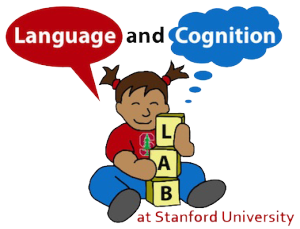
\includegraphics{figs/image-1} 

}

\caption[Field of view for three different headcam configurations, with the device we used in the middle]{Field of view for three different headcam configurations, with the device we used in the middle. The lowest camera is pictured for comparison, but was not available until after our study was already in progress.}\label{fig:image}
\end{figure}
\end{CodeChunk}

\subsection{Procedure}\label{procedure}

First, all parents signed consent documents in a waiting room where
children were fitted with the headcam. After the child was comfortable
in the waiting room and with the experimenter, the experimenter placed
the headcam on the child's head. If the child was uninterested in
wearing the headcam or tried to take it off, the experimenter presented
engaging toys to try to draw the child's focus away from the headcam
(Yoshida \& Smith, 2008).

After the child was comfortable with wearing the headcam, the child and
caregiver were shown to a playroom for the free-play session--the focus
of the current study. Parents were shown a box containing three pairs of
novel and familiar objects (e.g., a ball and a feather duster, named a
``zem''), and were instructed to play with the object pairs with their
child one at a time, ``as they typically would.'' All parents confirmed
that their child had not previosuly seen the novel toys and were
instructed to use the novel labels to refer to the novel toys.

The experimenter then left the playroom for approximately 15 minutes,
during which a tripod-mounted camera in the corner of the room recorded
the session and the headcam captured video from the child's perspective.

\subsection{Data Processing and
Annotation}\label{data-processing-and-annotation}

\begin{figure*}

\includegraphics[width=6in]{images/framesample.pdf}
\caption{\label{fig:frames} Example face detections made by MTCNN for the headcam videos from a child in each group  (green squares).}
\end{figure*}

Headcam videos were trimmed such that they excluded the instruction
phase when the experimenter was in the room and were automatically
synchronized with the tripod-mounted videos using FinalCut Pro Software.
These sessions yielded videos of 516 minutes (almost a milion frames),
with an average video length of 8.6 minutes (min = 4.53, max = 19.35).

\subsubsection{Posture and Orientation
Annotation}\label{posture-and-orientation-annotation}

We created a set of custom annotations that described the child's
physical posture (e.g.~standing) and the orientation of the caregiver
relative to the child (e.g.~far away). The child's posture was
categorized as being held/carried, prone (crawling or lying), sitting,
or standing. The caregiver's orientation was characterized as being
close to the child, farther from the child, and a global category of
caregiver behind the child. For the first two annotationes (close/far
from the child), the caregiver could either be to the the front or to
the side of the child. All annontations were made using
OpenSHAPA/Datavyu software (Adolph, Gilmore, Freeman, Sanderson, \&
Millman, 2012), and times when the child was out of view of the tripod
camera was marked as uncodable and was excluded from these annotations.

\subsection{Face Detection}\label{face-detection}

Measuring the availability of caregiver's faces across development was
an important goal of the study. We used a total of three face detection
systems to explore this hypothesis and to avoid the cost of
hand-annotating every frame. Results for the evaluation of these three
systems are shown in Table X.

\subsubsection{Face Detection
Algorithms}\label{face-detection-algorithms}

The first face detection system made use of a series of Haar
feature-based cascade classifiers (Viola-Jones, CITEXX) applied to each
individual frame. This detector provided information about the presence
of a face as well as its size and position.

The second algorithm was based on the work by (CITEXX) using multi-task
cascaded convolutional neural networks (MTCNNs). The system was built
using a novel cascaded CNN-based framework for joint detection and
alignment, built to perform well in real-world environments where
varying illuminations and occlusions are present. We used a Tensorflow
implementation of this algorithm provided by
(\url{https://github.com/davidsandberg/facenet})

The third algorithm was a CNN-based pose detector that provided the
locations of 18 body parts (ears, nose, wrists, etc) (CITEXX). The
system uses a CNN for initial anatomical detection and subsequently
applies part affinity fields (PAFs) for part association, producing a
series of body part candidates. The candidates are then matched to a
single individual and finally assembled into a pose. For the purposes of
our investigation we only made use of the body parts relevant to the
face (ears, eyes, nose).

\subsubsection{Detector evaluation}\label{detector-evaluation}

\begin{table}[t]
  \caption{Model performance on gold standard generalization training set dataset. P, R, and F denote precision, recall, and F-score for each of the two samples. \label{tab:model_eval}}
  \begin{center}
    \begin{tabular}{l|ccc|ccc}
      \hline
       &  \multicolumn{3}{c|}{High-density} &  \multicolumn{3}{c}{Random} \\
      % \null Model & P & R & F & P & R & F  \\
      \hline
      % Viola-Jones & .55  & .38 &  .45 & .89 & .74 & .81   \\
      % MTCNN & .86 & .78 & .81 & .93 & .76 & .83 \\
      % OpenPose-Faces & .86 & .78 & .81 & .93 & .76 & .83 \\
      % OpenPose-Wrists & .86 & .78 & .81 & .93 & .76 & .83 \\
      % OpenPose-Hands & .86 & .78 & .81 & .93 & .76 & .83 \\
    \hline
    \end{tabular}
  \end{center}
\end{table}

\section{Results}\label{results}

First, we report developmental shifts in infants' posture and their
orientation to their caregiver. Then, we explore how these changes
influence children's visual access to faces and to hands. Finally, we
explore how these changes impact the accessibility of faces and hands
during labeling events.

\section{Changes in Posture and
Orientation}\label{changes-in-posture-and-orientation}

\begin{CodeChunk}
\begin{figure}[H]

{\centering 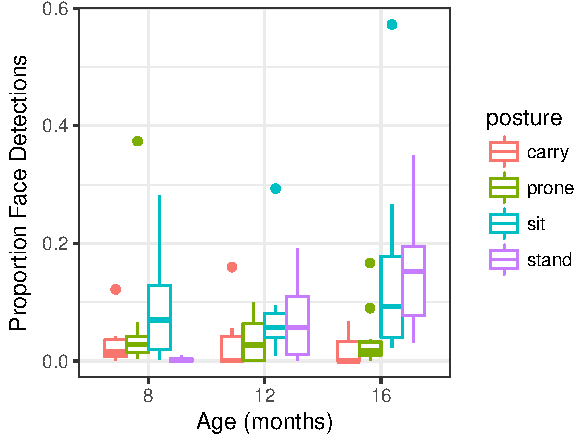
\includegraphics{figs/unnamed-chunk-4-1} 

}

\caption[R plot]{R plot}\label{fig:unnamed-chunk-4}
\end{figure}
\end{CodeChunk}

\section{Changes in Access to Faces}\label{changes-in-access-to-faces}

\begin{CodeChunk}
\begin{figure*}[h]

{\centering 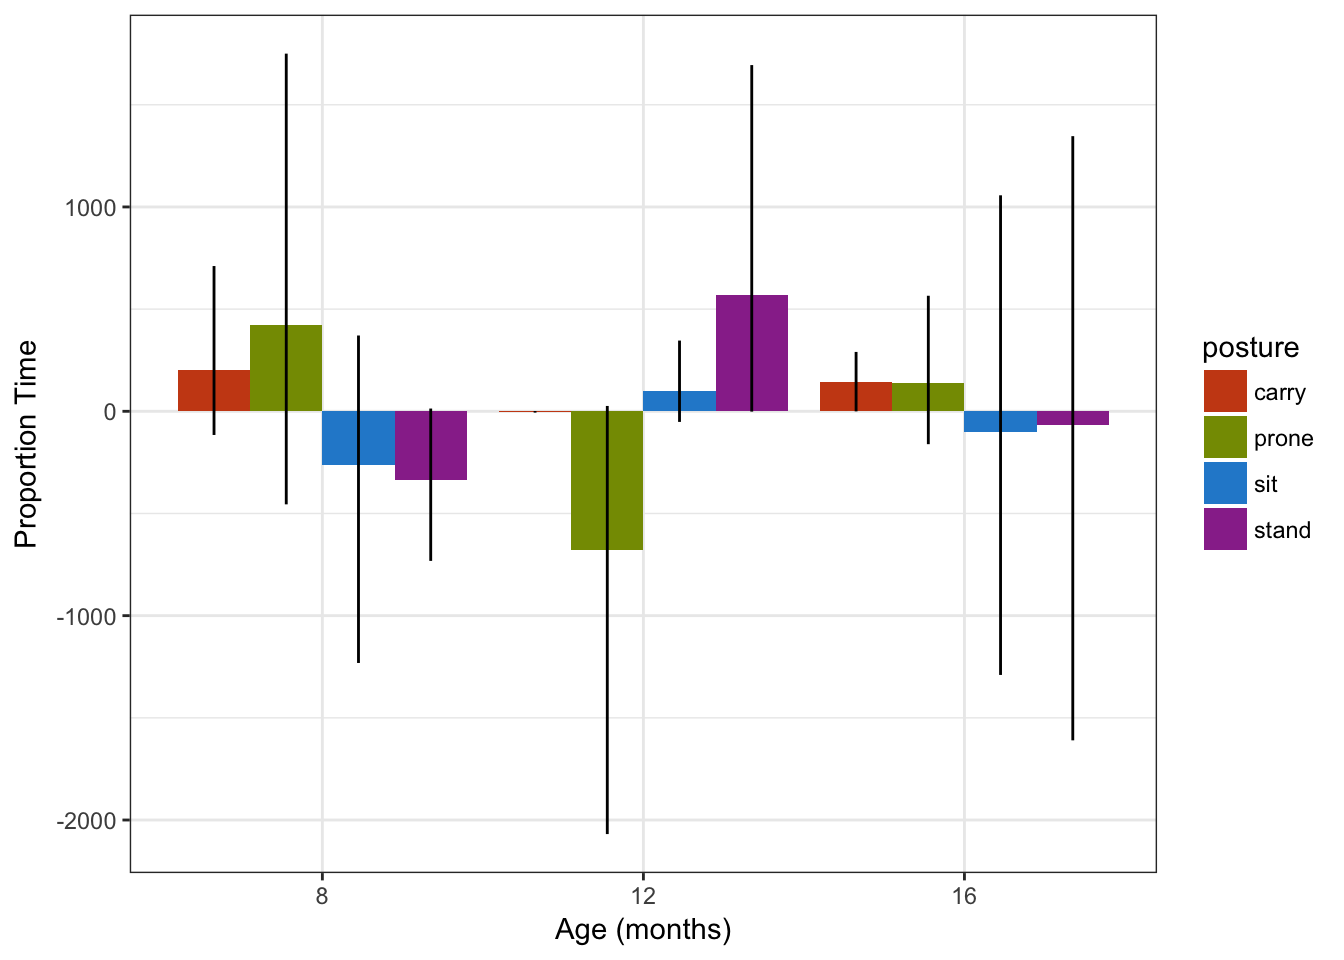
\includegraphics{figs/unnamed-chunk-5-1} 

}

\caption[Proportion face (left) and hand (right) detections as a function of participant's age]{Proportion face (left) and hand (right) detections as a function of participant's age. Note that the axes are different; hands were detected overall much less frequently in this dataset.}\label{fig:unnamed-chunk-5}
\end{figure*}
\end{CodeChunk}

\begin{CodeChunk}
\begin{figure*}[h]

{\centering \includegraphics{figs/faceByPostureFig-1} 

}

\caption[Proportion of face detections as a function of infant's posture, using the MTCNN3 detections (left panel) and OpenPose detections (right panel)]{Proportion of face detections as a function of infant's posture, using the MTCNN3 detections (left panel) and OpenPose detections (right panel)}\label{fig:faceByPostureFig}
\end{figure*}
\end{CodeChunk}

\begin{CodeChunk}
\begin{figure*}[h]

{\centering \includegraphics{figs/faceByOrientFig-1} 

}

\caption[Proportion of face detections as a function of caregiver's orientation,using the MTCNN3 detections (left panel) and OpenPose detections (right panel)]{Proportion of face detections as a function of caregiver's orientation,using the MTCNN3 detections (left panel) and OpenPose detections (right panel)}\label{fig:faceByOrientFig}
\end{figure*}
\end{CodeChunk}

To formalize these observations, we fit a generalized logistic
mixed-effect model to all with the presence/absence of a face on every
frame (as detected by the MTCNN3 model) as the dependent variable, and
participant's age, orientation, and posture as predictors. Interactions
between predictors were not included as this maximal model failed to
converge. A summary of the coefficients of this model can be found in
Table \{ref\}. While age remained a significant predictor even when
accounting for the effects of infants' posture and caregiver's
oirentation, it held relativley less predictive power. Overall, these
results confirm that infant's access to faces is heavily infleunced by
their own posture and their caregivers orientation towards them.

\begin{table}[H]
\centering
\begin{tabular}{rrrrr}
  \hline
 & Estimate & Std. Error & z value & Pr($>$$|$z$|$) \\ 
  \hline
(Intercept) & -4.846 & 0.077 & -62.682 & 0.000 \\ 
  Age & 0.170 & 0.061 & 2.766 & 0.006 \\ 
  Posture-Prone & -0.513 & 0.036 & -14.045 & 0.000 \\ 
  Posture-Sit & 0.648 & 0.034 & 18.853 & 0.000 \\ 
  Posture-Stand & 1.005 & 0.035 & 28.402 & 0.000 \\ 
  Orient.-Close & 1.549 & 0.021 & 72.757 & 0.000 \\ 
  Orient.-Far & 2.258 & 0.022 & 101.138 & 0.000 \\ 
   \hline
\end{tabular}
\caption{Results from GLMM model prediting the presence/absence of a face across                       the entire dataset.} 
\end{table}

\section{Changes in Access to Hands}\label{changes-in-access-to-hands}

Next, we examined whether we would see similar trends in infant and
children's access to hands.

\section{General Discussion}\label{general-discussion}

We use a head-mounted camera to explore how children's postural and
locomotive development directly impacts their access to social
information relevant for word-learning, here operationalized as the
presence of the faces and hands of their caregiver. We found that
children's posture and orientation towards their caregiver changed
systematically across age, and that all three of these factors
dramatically impacted the proportion of faces and hands that were
avaliable in the child's visual field. Thus, infants postural
development is mediating factor that explains age-related changes in the
proportion of faces and hands avaliable in infants' visual field.

This work also deploys novel advancements in computer vision to the
study of developmental psychology. The field of object detection and
recognition has advanced dramatically in the past five years since the
re-birth of deep learning algorithms (Krihevsky et al., 2012), creating
a new generation of algorithmic tools that both are substantially better
equipped to deal with noisier, more complicated datasets and that can
extract richer and more detailed information. Indeed, these videos from
the infant perspective provided sustantial challenges (e.g., partially
occluded faces) for the classc models of face detedction (e.g., viola
jones). Further, as the headcam technologies employed here were
inexpensive (\textasciitilde{}\$60 a camera) and the computer vision
algorithms freely avaliable, this method is a promising avenue for
quanitfying the visual and social information avaliable to new infant
learners.

Thus, we suggest that the combined use of these new tools can be
leveraged to understand the changing infant perspecive on the visual
world and the implications of these changes for both linguistic,
cognitive, and social development.

\section{Acknowledgements}\label{acknowledgements}

Thanks to Kaia Simmons, Kathy Woo, Aditi Maliwal, and other members of
the Language and Cognition Lab for help in recruitment, data collection,
and annotation. This research was supported by a John Merck Scholars
grant to MCF. An earlier version of this work was presented to the
Cognitive Science Society in Frank, Simmons, Yurovsky, \& Pusiol (2013).
Please address correspondence to Michael C. Frank, Department of
Psychology, Stanford University, 450 Serra Mall (Jordan Hall), Stanford,
CA, 94305, tel: (650) 724-4003, email: \texttt{mcfrank@stanford.edu}.

\section{References}\label{references}

\setlength{\parindent}{-0.1in} \setlength{\leftskip}{0.125in} \noindent

\hypertarget{refs}{}
\hypertarget{ref-adolph2007}{}
Adolph, K., \& Berger, S. (2007). Motor development. In \emph{Handbook
of child psychology}. Wiley Online Library.

\hypertarget{ref-adolph2012}{}
Adolph, K., Gilmore, R., Freeman, C., Sanderson, P., \& Millman, D.
(2012). Toward open behavioral science. \emph{Psychological Inquiry},
\emph{23}(3), 244--247.

\hypertarget{ref-brooks2005}{}
Brooks, R., \& Meltzoff, A. (2005). The development of gaze following
and its relation to language. \emph{Developmental Science}, \emph{8}(6),
535--543.

\hypertarget{ref-carpenter1998}{}
Carpenter, M., Nagell, K., \& Tomasello, M. (1998). Social cognition,
joint attention, and communicative competence from 9 to 15 months of
age. \emph{Monographs of the Society for Research in Child Development},
\emph{63}(4).

\hypertarget{ref-cummings1988}{}
Cummings, M., Van Hof-Van Duin, J., Mayer, D., Hansen, R., \& Fulton, A.
(1988). Visual fields of young children. \emph{Behavioural and Brain
Research}, \emph{29}(1), 7--16.

\hypertarget{ref-franchak2011}{}
Franchak, J., Kretch, K., Soska, K., \& Adolph, K. (2011). Head-mounted
eye tracking: A new method to describe infant looking. \emph{Child
Development}.

\hypertarget{ref-frank2013}{}
Frank, M. C., Simmons, K., Yurovsky, D., \& Pusiol, G. (2013).
Developmental and postural changes in children’s visual access to faces.
In \emph{Proceedings of the 35th annual meeting of the cognitive science
society} (pp. 454--459).

\hypertarget{ref-mayer1988}{}
Mayer, D., Fulton, A., \& Cummings, M. (1988). Visual fields of infants
assessed with a new perimetric technique. \emph{Investigative
Ophthalmology \& Visual Science}, \emph{29}(3), 452--459.

\hypertarget{ref-walle2014}{}
Walle, E. A., \& Campos, J. J. (2014). Infant language development is
related to the acquisition of walking. \emph{Developmental Psychology},
\emph{50}(2), 336.

\hypertarget{ref-yoshida2008}{}
Yoshida, H., \& Smith, L. (2008). What's in view for toddlers? Using a
head camera to study visual experience. \emph{Infancy}, \emph{13},
229--248.

\hypertarget{ref-yurovsky2012}{}
Yurovsky, D., Smith, L., \& Yu, C. (in press). Statistical word learning
at scale: The baby's view is better. \emph{Developmental Science}.

\end{document}
